\documentclass[12pt]{article}
\usepackage{amsmath}
\usepackage{graphicx}
\usepackage{wrapfig}
\usepackage{booktabs}
\usepackage[letterpaper, margin=1in]{geometry}
\usepackage{fancyhdr}
\pagestyle{fancy}
\fancyhead[R]{The Operational Amplifier}
\fancyfoot[C]{\thepage}
\renewcommand{\headrulewidth}{1pt}
\renewcommand{\footrulewidth}{1pt}
\usepackage [autostyle, english = american]{csquotes}
\MakeOuterQuote{"}
\renewcommand{\baselinestretch}{1.0}
\newcommand{\twoobjects}[2]{%
  \leavevmode\vbox{\hbox{#1}\nointerlineskip\hbox{#2}}%
}
\begin{document}
    \section*{General Information}
    \begin{figure}[h]
        \centering
        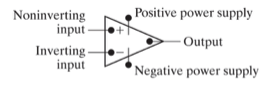
\includegraphics[width=0.4\textwidth]{Op-Amp.png}
    \end{figure}
    \par The purpose of an operational amplifier is to amplify the incoming
    input voltage by some linear amount. The amplifier possesses a saturation
    point at which the voltage is no longer amplified. This is based on the
    voltage of the power supply that is connected to the device. Since there is
    an attached power supply, the device is considered non-passive and it
    explains the limits of the linear behavior of the device which spans from
    $-V_{cc}$ to $V_{cc}$.
    \par For an ideal op-amp, the inverting and non-inverting voltage will be
    equal since the resistance within the amplifier is, ideally infinite, no
    current will flow through the actual device, $v_n = v_p$.
    \begin{figure}[h]
        \centering
        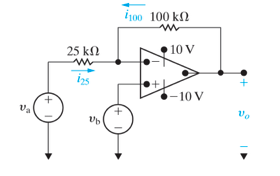
\includegraphics[width=0.4\textwidth]{Op-Amp Example Circuit.png}
    \end{figure}
    \par This example circuit can be analyzed to find the output voltage and
    thus the amplification that the device provides. Using $v_a = 1\ V$ and $v_b
    = 2\ V$, node equations can be written for the inverting node and the output
    node to determine the value of $v_0$. Since $v_n = v_p$, and the voltage at
    non-inverting input is simply $v_b$, the voltage at the node of the
    inverting input will also be equal to the voltage $v_b$. The first node
    equation therefore will be,
    \[
        \frac{v_b-v_a}{25000} + \frac{v_b-v_0}{100000} = 0
    \]
    \par Solving this equation by plugging in the values for $v_a$ and $v_b$,
    the value of $v_0$ is found to be $6\ V$. Since $V_{cc}$ ranges from $-10\
    V$ to $10\ V$, and the value of $v_0$ was found to be $6\ V$, this amplifier
    is operating within its linear region.
    \par We can also determine the range for which this amplifier can operate
    within its linear region by substituting the constraint values of $V_{cc}$
    in for $v_0$ and solving for $v_b$. Arranging the equation to solve for
    $v_b$,
    \[
        v_b = 20000(\frac{v_a}{25000} + \frac{v_0}{100000}) =\frac{4}{5}v_a +
        \frac{1}{5}v_0
    \]
    \par Now, plugging in $10\ V$ for $v_0$, the upper bound for $v_b$ is $2.8\
    V$ and the lower bound, from plugging in $-10\ V$, equals $-1.2\ V$,
    therefore, the linear operating range for this particular amplifier must
    respect, $-1.2\ V \le v_b \le 2.8\ V$.
    \section*{The Inverting-Amplifier}
    \begin{figure}[h]
        \centering
        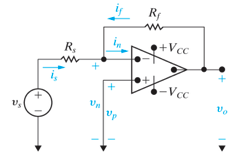
\includegraphics[width=0.4\textwidth]{Inverting Amplifier.png}
    \end{figure}
    \par This is circuit for the inverting amplifier and it is called such due
    to the source voltage being connected to the inverting input node of the
    device. The resulting behavior is that the output voltage is negative for
    any positive input voltage. Using the node equations once again as done with
    all of these circuits, here the voltage of the left node is zero since the
    non-inverting input is connected directly to ground, $v_n = 0$ and since
    $v_p = v_n$, $v_p = 0$. Solving the node equations as done previously, an
    expression for $v_0$ can be written,
    \[
        v_0 = -\frac{R_f}{R_s}v_s
    \]
    \par The amount of amplification received here will be equal to the
    fractional term, $\frac{R_f}{R_s}$. To find the range of values for $v_s$
    that will satisfy the linear behavior of the device, the same method can be
    employed as before, plugging in $V_{cc}$ for $v_0$ and solving for $v_s$.
    \section*{The Summing Amplifier}
    \begin{figure}[h]
        \centering
        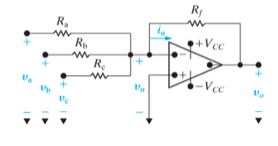
\includegraphics[width=0.4\textwidth]{Summing Amplifier.png}
    \end{figure}
    \par The circuit for the summing amplifier is shown and consists of multiple
    input sources, dampened by resistors, and all connected to the inverting
    input of the op-amp.
    \par The equation for the output voltage for this configuration is given by,
    \[
        v_0 = -\left( \frac{R_f}{R_a}v_a + \frac{R_f}{R_b}v_b +
        \frac{R_f}{R_c}v_c \right)
    \]
    \par If the input resistors are all equivalent, $R_a = R_b = R_c$, the
    equation can be written simply as the functional resistance over the source
    resistance, $R_s$,
    \[
        v_0 = -\frac{R_f}{R_s}(v_a + v_b + v_c)
    \]
    \section*{The Non-Inverting Amplifier}
    \begin{figure}[h]
        \centering
        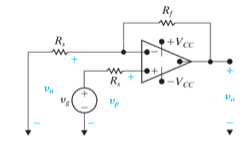
\includegraphics[width=0.4\textwidth]{Non-Inverting Amplifier.png}
    \end{figure}
    \par For this circuit it can be seen that the input voltage is connected to
    the non-inverting input of the op-amp therefore, this is a non-inverting
    amplifier. Functioning very similarly to the inverting amplifier, the
    equation can be found to be very similar as well.
    \[
        v_0 = \frac{R_s + R_f}{R_s}v_g
    \]
    \begin{center}
        \textit{or,}
    \end{center}
    \[
        v_0 = \left( 1 + \frac{R_f}{R_s} \right)v_g
    \]
    \par Using one of these equations will yield the value of $v_0$ and the
    amount of amplification that the amplifier provides. It also gives the
    region of linearity with the expression,
    \[
        \left( 1 + \frac{R_f}{R_s} \right) <\ \mid \frac{V_{cc}}{v_g} \mid
    \]
    \section*{The Difference Amplifier}
    \begin{figure}[h]
        \centering
        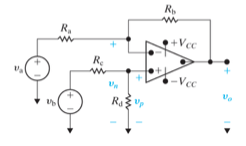
\includegraphics[width=0.4\textwidth]{Difference Amplifier.png}
    \end{figure}
    \par The last iteration of the operational amplifier and it is difference
    amplifier. This will take in two sources at both inputs as well as a path to
    ground which is connected to the non-inverting side of the amplifier. To
    find the equation of the output voltage in this case requires the same
    procedure as the others, the node equations an be written for the two nodes.
    In some cases however, if the resistor connected to the non-inverting input is
    not directly connected to the node, the voltage source $v_b$, may be
    converted to a Thevenin's equivalent circuit, which then gives a source in
    series with a resistor, and the equations can be written and solved.
    \[
        v_0 = \frac{R_d(R_a + R_b)}{R_a(R_c + R_d)}v_b - \frac{R_b}{R_a}v_a
    \]
    \par This equation can be simplified drastically however, it requires a few
    conditions to hold true in order to do so. If $\frac{R_a}{R_b} =
    \frac{R_c}{R_d}$, the equation can be written as,
    \[
        v_0 = \frac{R_b}{R_a} (v_b - v_a)
    \]
    \par With all the resistors given along with the two input sources, the
    output voltage can be determined and with that, as can be the range of the
    input voltage for the linear operation of the amplifier.
\end{document}
